\chapter{System Concept}\label{chap:concept}
The following chapter will cover the system concept, the functionality it offers and the general functional system description. Also, the following sections should clarify how the SmartNotes application can be used, illustrate its design using the UML diagrams and prepare the reader for more detailed system description included in the chapter~\ref{chap:sys_description}.

The idea of SmartNotes has been inspired by the Google Notebook application which was being actively developed until January 2009, when Google announced that further development work on this project is stopped. Google Notebook has an interesting interface and features, some of them already motioned in section~\ref{subsec:google_notebook}. what was still missing from the functionality until January 2009 was comfortable notes usage without network connectivity. The aim of the subject of the thesis was to use the idea of making a truly scalable notes taking application that would be even more flexible.

\section{Functionality description}\label{sec:functionality_descr} 
Detailed description of how a system may be used should by of utmost importance both to the developer and to the end user, as it helps gain a general perspective, called 10,000-foot view\cite[page 49]{uml_use_case}, of the system and make useful observations. The implementation as well as the conceptual and system design decisions become a side issue, as the foreground is always occupied by the functionality  the application is to offer. For that reason, the use of case scenarios and flow charts will be very helpful in describing the efficient way of using the SmartNotes application.

Users willing to work on their notes disregarding network connectivity will need to install iSmartNotes, which is a graphical interface of SmartNotes. Specifically, the SmartNotes application is divided into the web-based system and the graphical desktop interface, a separation with which UI experiments can be done without the need of having the web browser open in order to work on the notes. The web based part of SmartNotes makes the synchronization feature possible and allows to monitor the entire system of SmartNotes. However, in order to use the synchronization feature, the iSmartNotes needs to be activated by the user. Additionally, since users of SmartNotes are expected to have a Google account\footnote{Creating a Google account by visiting \url{https://www.google.com/accounts/} gives a access to various services offered by the Google company where Gmail, Google News or Google Finance are one of the most popular tools. These are regarded secure and solid services users can relay on.} the activation code will be available after logging in to the SmartNotes system with that account. This process is illustrated on figure~\ref{fig:ismartnotes_activation}. The idea behind it is to make the use of the popular Google Account and not multiply the accounts to services that the user has to know the login and password. Basing on the activation key, the user is granted access to his personalized SmartNotes account and to the synchronization feature. Without the activation, iSmartNotes can be used as a regular notes editor.  
\begin{figure}[ht]
\begin{center}
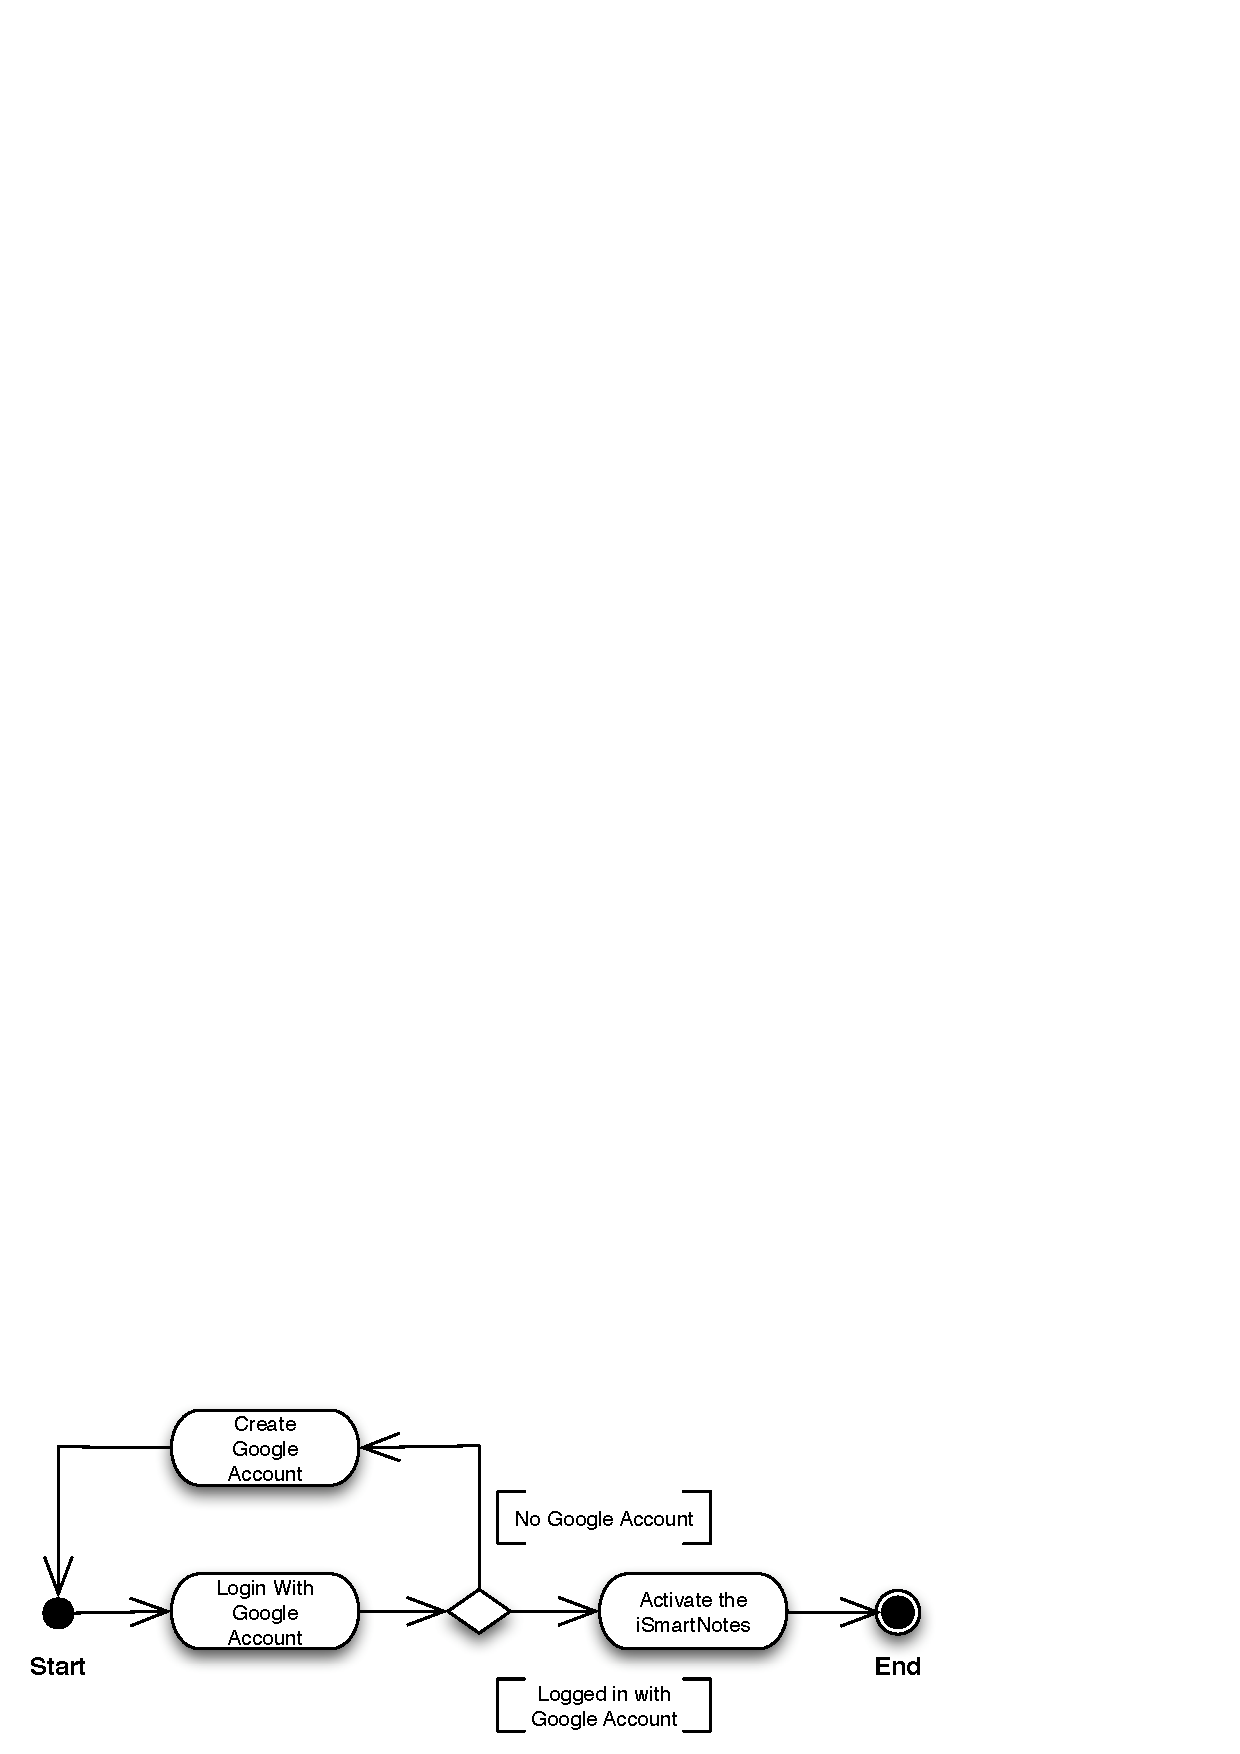
\includegraphics[scale=0.65]{charts/activate_iSmartNotes.png}
\caption{The iSmartNotes application activation with the Google Account.}
\label{fig:ismartnotes_activation}
\end{center}
\end{figure}
The skim of functionality offered by iSmartNotes is demonstrated on figure~\ref{fig:workon_ismartnotes}.
\begin{figure}[ht]
\begin{center}
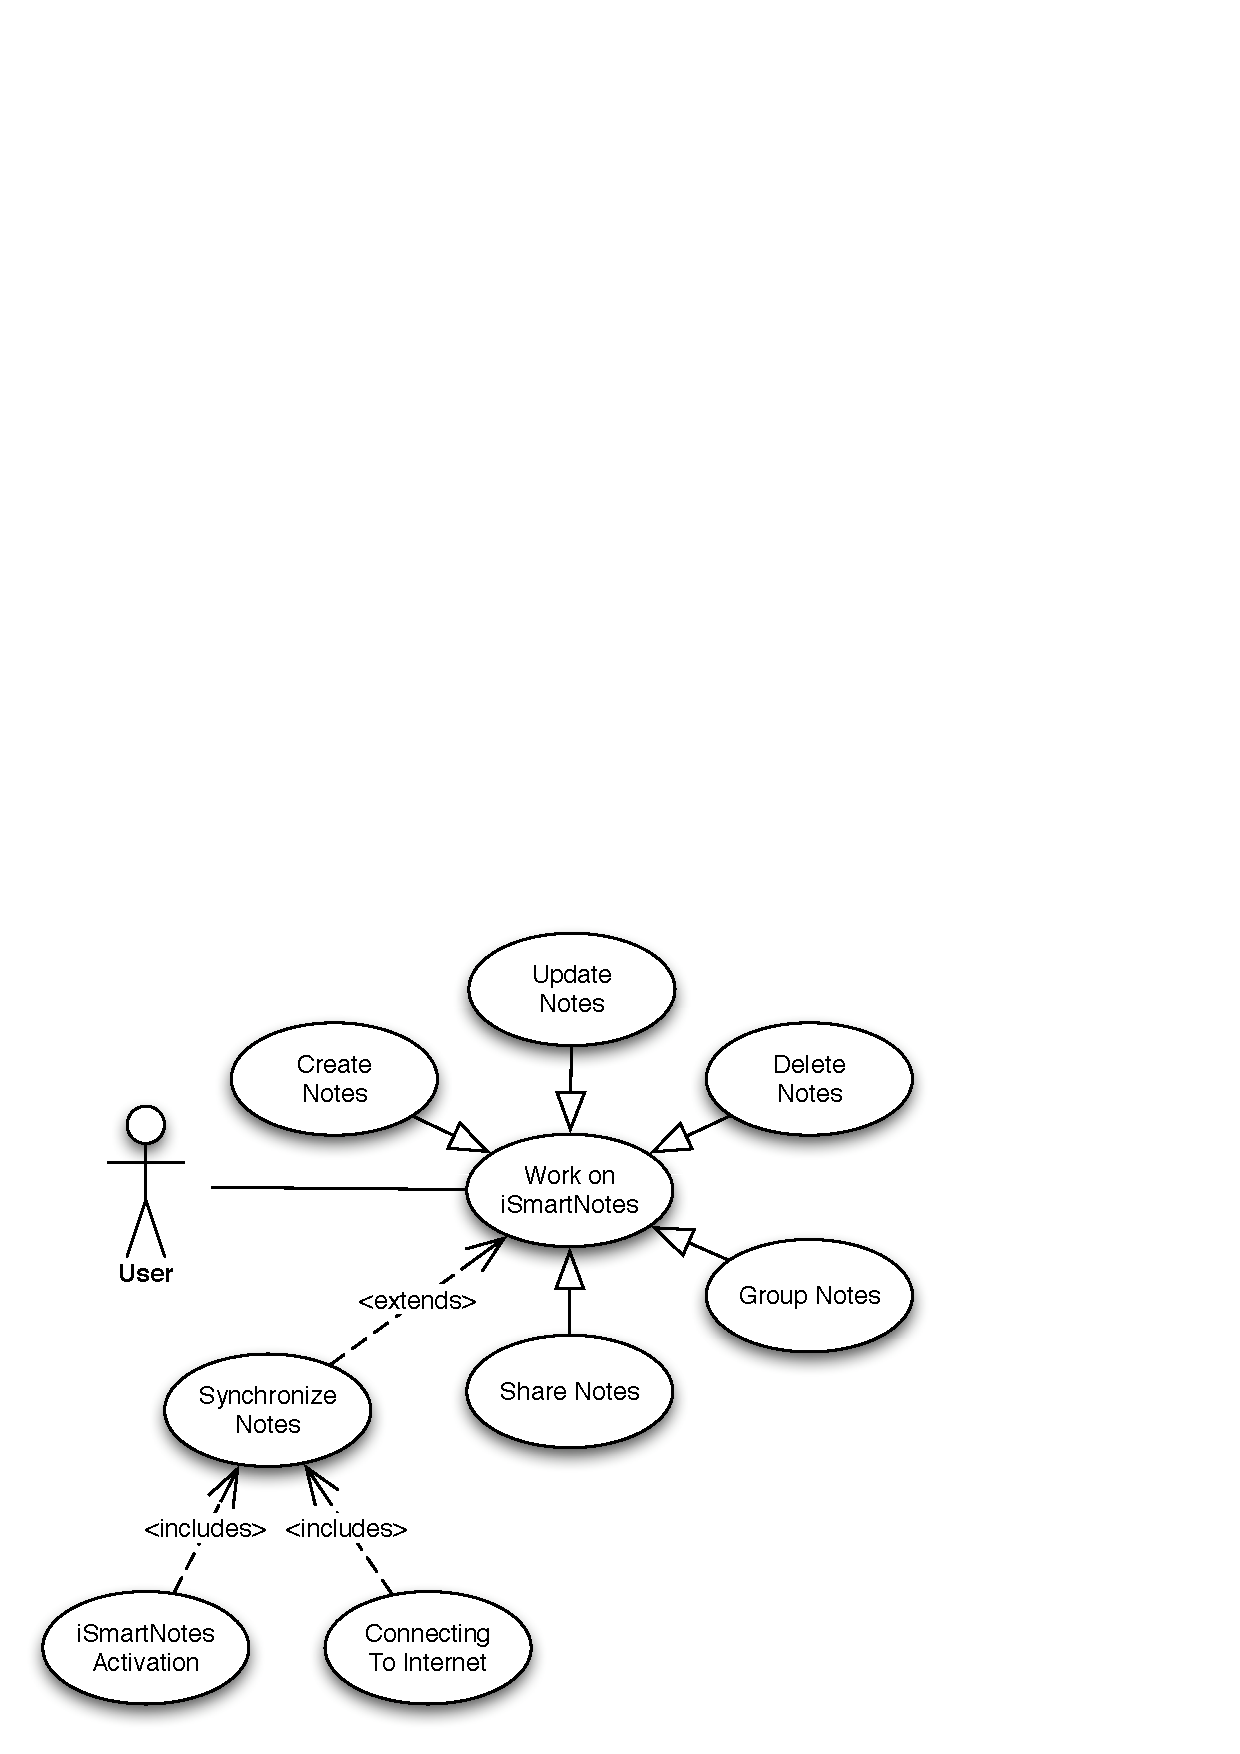
\includegraphics[scale=0.55]{charts/work_on_iSmartNotes.png}
\caption{The iSmartNotes application use cases.}
\label{fig:workon_ismartnotes}
\end{center}
\end{figure}
This includes the CRUD operations and three extra features. Firstly, the notes can be easily grouped together in named tabs, which should make organizing and finding notes much easier. Secondly, it is possible to publish the notes marked as shared. The final feature is the synchronization process that requires iSmartNotes activation and network connection to contact with the web-based part of SmartNotes. What remains to be discussed is the cooperation between iSmartNotes and the web-based part of SmartNotes, therefore, the relation between them and the functionality offered to the user and administrator are shown on figure~\ref{fig:ismartnotes_smartnotes}. 
\begin{figure}[ht]
\begin{center}
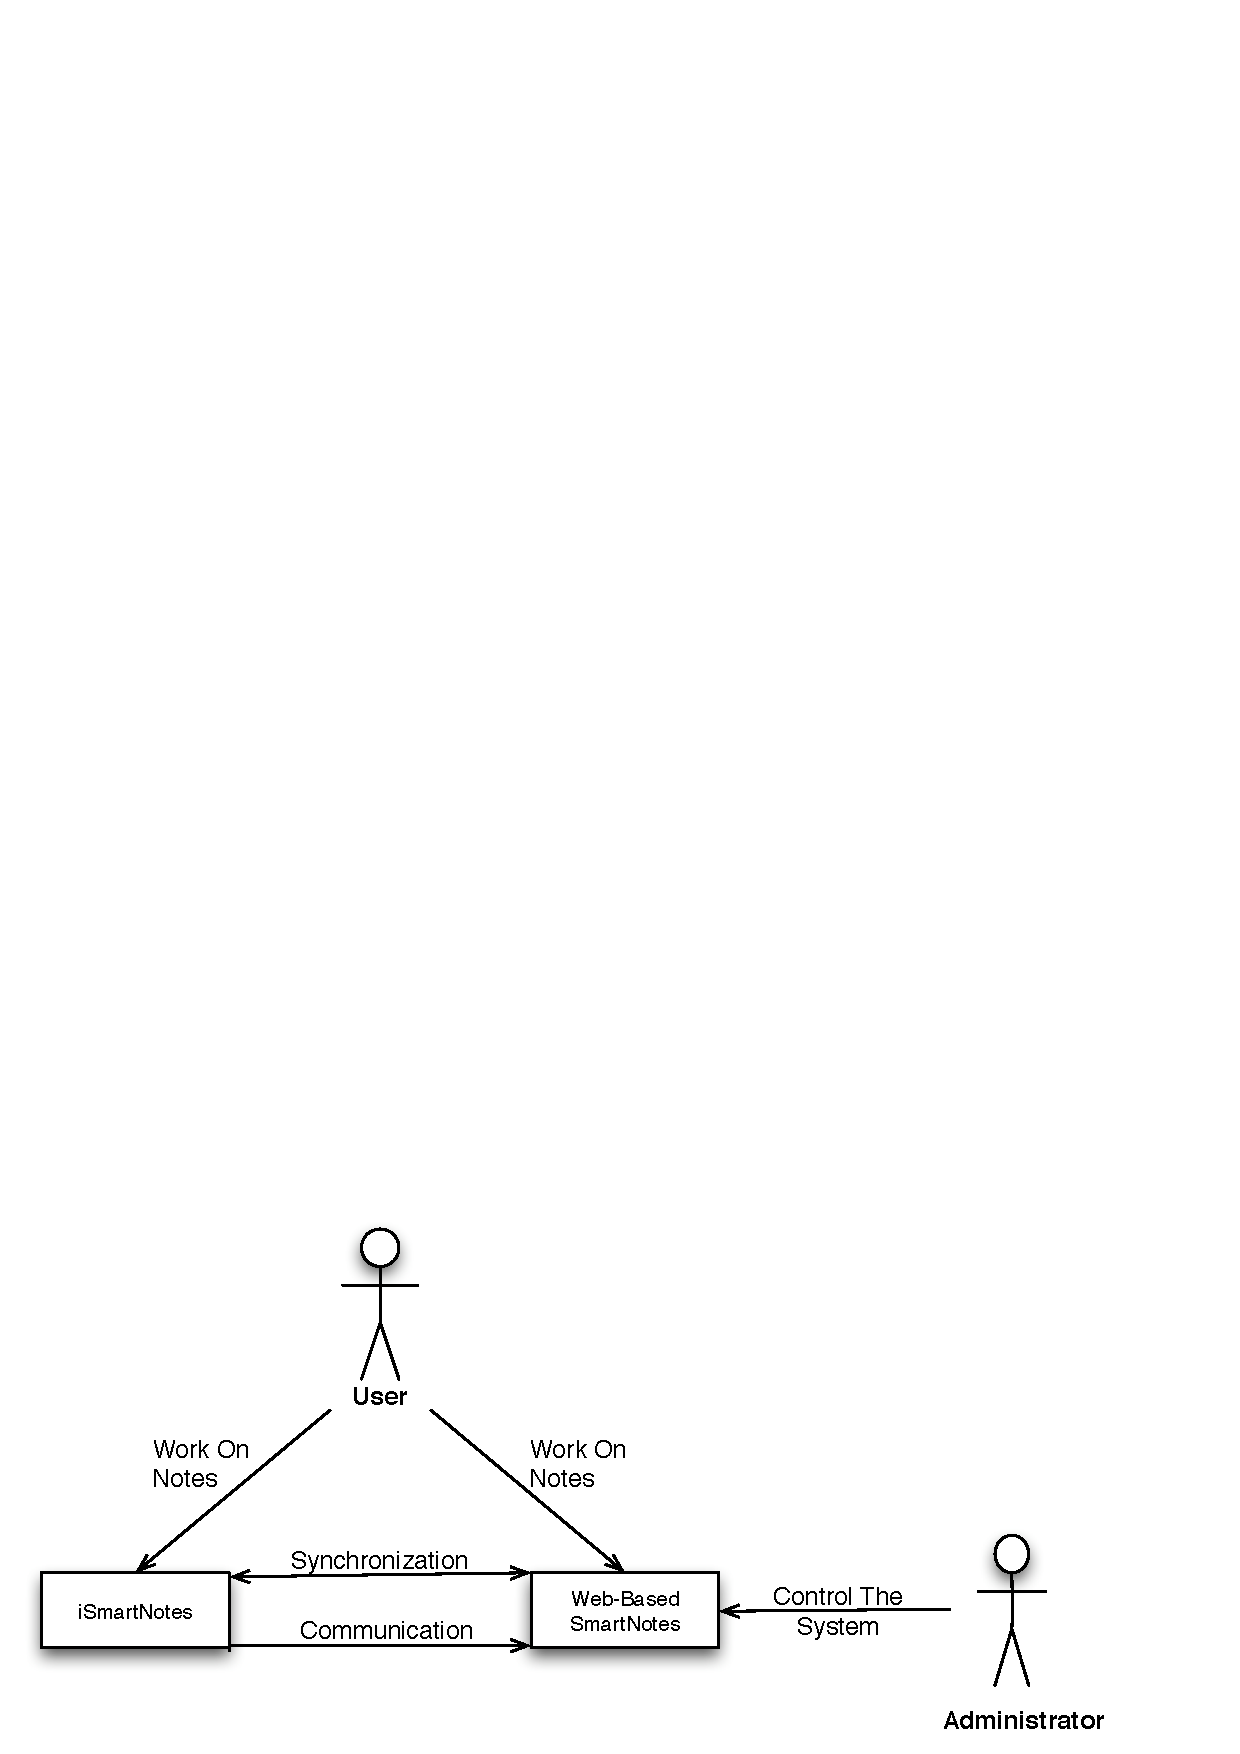
\includegraphics[scale=0.55]{charts/iSmartNotes_SmartNotes.png}
\caption{The cooperation of iSmartNotes and web based SmartNotes.}
\label{fig:ismartnotes_smartnotes}
\end{center}
\end{figure}

*****It is interesting concept to allow the user work on iSmartNotes and on the Web based part of SmartNotes exchangeably  and letting the SmartNotes application care for work synchronization. This was also marked on the discussed picture. However that is a remark of what could be done to make the application more functional and elastic but the user functionality of the web interface of realized project will be mineralized. On the Other hand administrator will get the access to such a tools like datastore data browser, system status or application dashboard described in section~\ref{sec:gae_general}. This can help to fast diagnose that something is going not right with the application and rollback it to the latest stable version. Moreover  it can indicate that the rescuers are not sufficient to serve the traffic and eventually extend them. Those tools work great with cooperation with Google Webmaster Tools and the Google Analytics as they can provide more information concerning the web page and its visitors.

Some additional explanations requires the synchronization feature. It will be realized by the version control system which were introduced in section~\ref{sec:popular_vcs}. No matter if the user works online or not he will have the full access to his notes and when he can use Internet notes can become synchronized. As marked on the graph from figure~\ref{fig:ismartnotes_smartnotes} the synchronization process is bidirectional from the web based part of SmartNotes which plays a role of main server and the iSmartNotes playnig the role of clients and reverse. That should allow to update the notes which could be for example edited just before leaving the office or push the just added list of things to do after coming from vacation. Next thing marked on the graph from figure~\ref{fig:ismartnotes_smartnotes} is the one directional communication between iSmartNotes and SmartNotes which should be understand as a additional logic allowing the to perform some operations on the user side by the help of iSmartNotes. That should include displaying the user information's about some important events like availability of new feature or information about availability of newer version.  Its one directional as it will be iSmartNotes application which will be in order to get this informations from the SmartNotes server and display it to the user. The presented functionality definitely does not fully exploit the possible feature list but as mentioned in section~\ref{subsec:vcs_comparison} it is a good practice to keep the application as simple as possible and focus on a set of clearly defined key features.

\section{Functional description}\label{sec:functional_descr}
The SmartNotes application should run on a infrastructure that can ensure high availability and that is ready to handle high load. Easy system maintenance and being open for future functionality expanding are also strongly desirable features. It is not pointless to mention that all this requires resource usage what means that financial model is really on importance. That is a developer 10,000-foot view for the system requirements. Adding a friendly deployment methodology and good documentation it is what would make even the most demanding developer smile.

Users should get well informed about the application, what it does and be able to easily find instructions how to get started. For those reasons the landing page should be informal and practical. It would be best if it wold be international to reach greater group of users.

From the architectural point of view SmartNotes are though as a simple client-server application. A small difference is that SmartNotes uses DVCS which makes all using it the machines access same set of commands and make their hard disks hold the entire repository with it history. It may be confusing that it still remains a client-server architecture. In dead it is a little strange but just like centralized VCS don't know any other architecture than client-server the distributed version control systems uses it as one of possible use cases. In fallowing scenario one of the machines fulfills a role of reverential server to which all remaining machines direct their requests. It is a kind of public repository with the most recent version that should be always available to the others. In consequence each client needs installing DVCS as one of main components. Therefore the size of chosen VCS matters almost just as much as it performance which will significantly determine the final performance of iSmartNotes. For optimum user experience the iSmartNotes application should be served easy to instal package that could be downloaded from server serving static content. This is not only a faster solution from dynamically served content but also allows to save on system resources as it does cost minimum of CPU time.

The next two sections state some interesting problems synchronization scenarios using VCS and the application activation. They will be analyzed focussing on evaluating some of possible solutions. Finally the best possible to implement idea will be chosen.  
 
\subsection{Synchronization scenarios using version control systems}\label{subsec:sync_scenarios}
It is one of the roles of version control systems to keep the repositories updated. Nevertheless they never make it without the user request\footnote{This means that the user has to run appropriate command or click on the right button when using a graphical interface. It could be naturally automated by writing some script that would perform that task for user or by setting a cron job with desired time interval but it still needs user to trigger the update process.}. That may be from several reasons among which dealing with conflict situation like shown on figure~\ref{fig:google_notebook} seams to be the most important. To put in simple words it is a situation when the VCS needs the user decision to resolve the conflict situation. The way the merging is done also differs with different version control systems but from the user perspective operations such like update and merge are easy to imagine when basing on the their final result. It is also some mix of terminology including this basic operations. Fetch implemented by git system consists of three steps:
\begin{enumerate}
\item{lookup}
\item{getting changes}
\item{updating or merging}
\end{enumerate}
\subsection{iSmartNotes activation process}\label{subsec:ismartnotes_activation}
